 % !TEX TS-program = pdflatex
% !TEX encoding = UTF-8 Unicode



\documentclass[slidetop,11pt]{beamer}

\usepackage[francais]{babel}
\usepackage[T1]{fontenc}
\usepackage[utf8]{inputenc}

\usepackage{amsmath,amsfonts,amssymb,ulem,epigraph}

\usepackage[upright]{fourier}

\usepackage{shadethm}

\usepackage{subfig}

\usepackage{pgf,tikz}
\usetikzlibrary{arrows}

\usepackage{color}
\definecolor{gris_clair}{gray}{.9}
\definecolor{gris}{gray}{.35}
\definecolor{vert}{rgb}{0,0.5,0}
\definecolor{rouge}{rgb}{0.5,0,0}
\definecolor{turquoise}{rgb}{0,0.5,0.5}

%\graphicspath{{./} {./experience/utiliteordrecontrainte/}}

\usepackage{listings}           
\lstset{
language=Caml,
backgroundcolor=\color{gris_clair},
frame=single,
basicstyle=\footnotesize\ttfamily\color{gris},
identifierstyle=\color{black},
keywordstyle=\color{vert},
stringstyle=\color{rouge}, showstringspaces=false,
commentstyle=\itshape\color{turquoise},
%numbers=left, numbersep=5pt, numberstyle=\color{gris}\tiny,stepnumber=5,
breaklines=true,
literate=
  {é}{{\'e}}1 {É}{{\'E}}1 {à}{{\`a}}1 {è}{{\`e}}1% 
  {À}{{\`A}}1 {È}{{\'E}}1 {ë}{{\"e}}1 {ï}{{\"i}}1%
  {â}{{\^a}}1 {ê}{{\^e}}1 {î}{{\^i}}1 {ô}{{\^o}}1% 
  {û}{{\^u}}1 {Â}{{\^A}}1 {Ê}{{\^E}}1 {Î}{{\^I}}1%
  {Ô}{{\^O}}1 {œ}{{\oe}}1 {Œ}{{\OE}}1 {æ}{{\ae}}1%
  {Æ}{{\AE}}1 {ç}{{\c c}}1 {Ç}{{\c C}}1 {€}{{\EUR}}1 ,
morekeywords={len,input,range}}

\usetheme{Warsaw}
\usecolortheme{beaver}

\graphicspath{{./} {./../source/}}

\title{Le Manège enchanté}
\date{}
\author{Antonin Dudermel}

\begin{document}

\newshadetheorem{defin}{Définition}
\newshadetheorem{theo}{Théorème}

\frame{\titlepage}

\begin{frame}
	\epigraph{Arrête de tourner en rond : détermine tes priorités, dégage les grands axes, et accélère !}{\it Alban}
\end{frame}

\begin{frame}
	\tableofcontents
\end{frame}

\begin{frame}
	\section{Le Manège enchanté}
	\begin{center}
		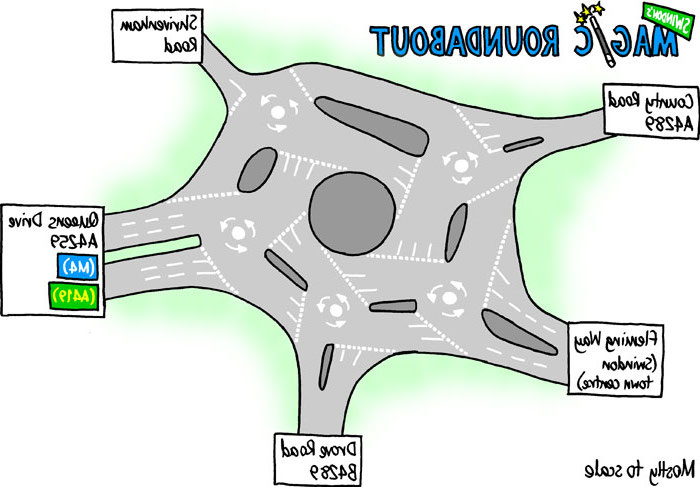
\includegraphics[scale=0.4]{magic}
	\end{center}
\end{frame}

\begin{frame}
	Fonctionnement :
	\begin{itemize}
		\item 1 grand rond-point central tournant dans le sens inverse
		\item 5 petits rond-points latéraux
		\item Des lignes de "cédez le passage" avec de l'espace pour plusieurs voitures
	\end{itemize}
\end{frame}

\begin{frame}
	Les prétentions du manège :
	\begin{itemize}
		\item diminuer la distance de trajet
		\item plus efficace
		\item moins d'accidents
	\end{itemize}
\end{frame}

\section{Caractériser le trafic}
	\subsection{Mesures}
\begin{frame}
	\frametitle{Mesures empiriques}
	Moyens :
	\begin{itemize}
		\item boucles magnétiques
		\item caméras
	\end{itemize}
\end{frame}

\begin{frame}
	\frametitle{Grandeurs}
	\begin{itemize}
		\item flux $J \text{ en } \mathrm{veh}/\mathrm{s}$
		\item vitesse $v \text{ en } \mathrm{m}/\mathrm{s}$
		\item densité $\rho \text{ en } \mathrm{veh}/\mathrm{m}$
	\end{itemize}
	$$J = \rho<v>$$
\end{frame}

\begin{frame}
	\begin{figure}
	\begin{center}
	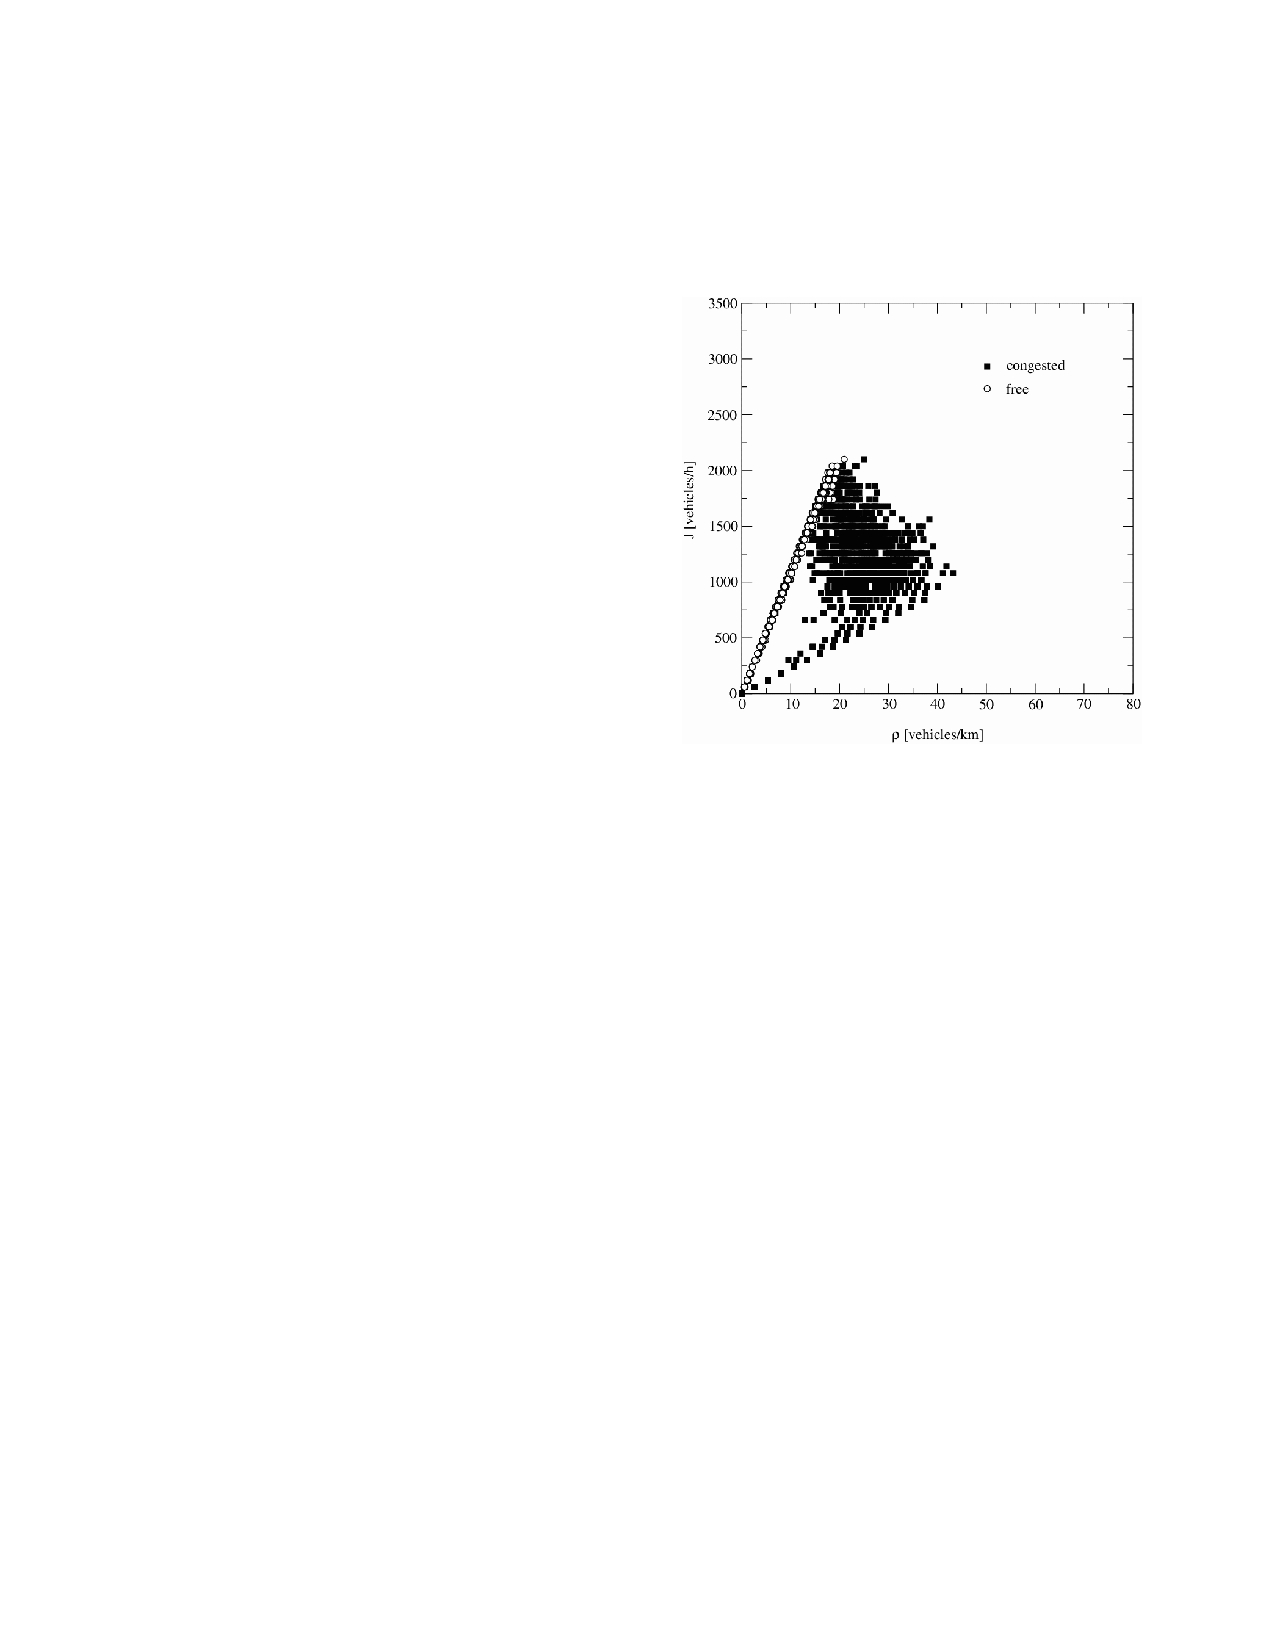
\includegraphics[scale = 0.7]{diagramme-fondamental}
	\end{center}
	\caption{diagramme fondamental}
	\end{figure}

\end{frame}

	\subsection{Différents trafics}
\begin{frame}
	\frametitle{Différents trafics}
	flot libre/flot synchronisé/embouteillages
\end{frame}

\section{Modéliser un rond-point}
\subsection{ Modéliser une section de route}
\begin{frame}
	\frametitle{Modèle Nagel-Schreckenberg (NaSch)}
	\begin{enumerate}
		\item Accélération 
		\item Décélération
		\item Facteur aléatoire
		\item Mouvement
	\end{enumerate}
\end{frame}

\begin{frame}
	\frametitle{Accélération}
	Avec $v_i$ la vitesse de la voiture $i$, $v_{max}$ la vitesse maximale autorisée : 
	\begin{equation}
		v_i \leftarrow \min (v_i+1,v_{max})
	\end{equation}
\end{frame}

\begin{frame}
	\frametitle{Décélération}
	avec $d_i$ la distance entre les voitures $i$ et $i+1$
	\begin{equation}
		v_i \leftarrow \min (v_i,d_i-1)
	\end{equation}
\end{frame}

\begin{frame}
	\frametitle{Facteur aléatoire}
	\begin{equation}
		v_i \leftarrow \max(v_i-1,0) \text{ avec proba } p
	\end{equation}
\end{frame}

\begin{frame}
	\frametitle{Mouvement}
	\begin{equation}
		x_i \leftarrow x_i + v_i
	\end{equation}
\end{frame}

\begin{frame}
\frametitle{validité}
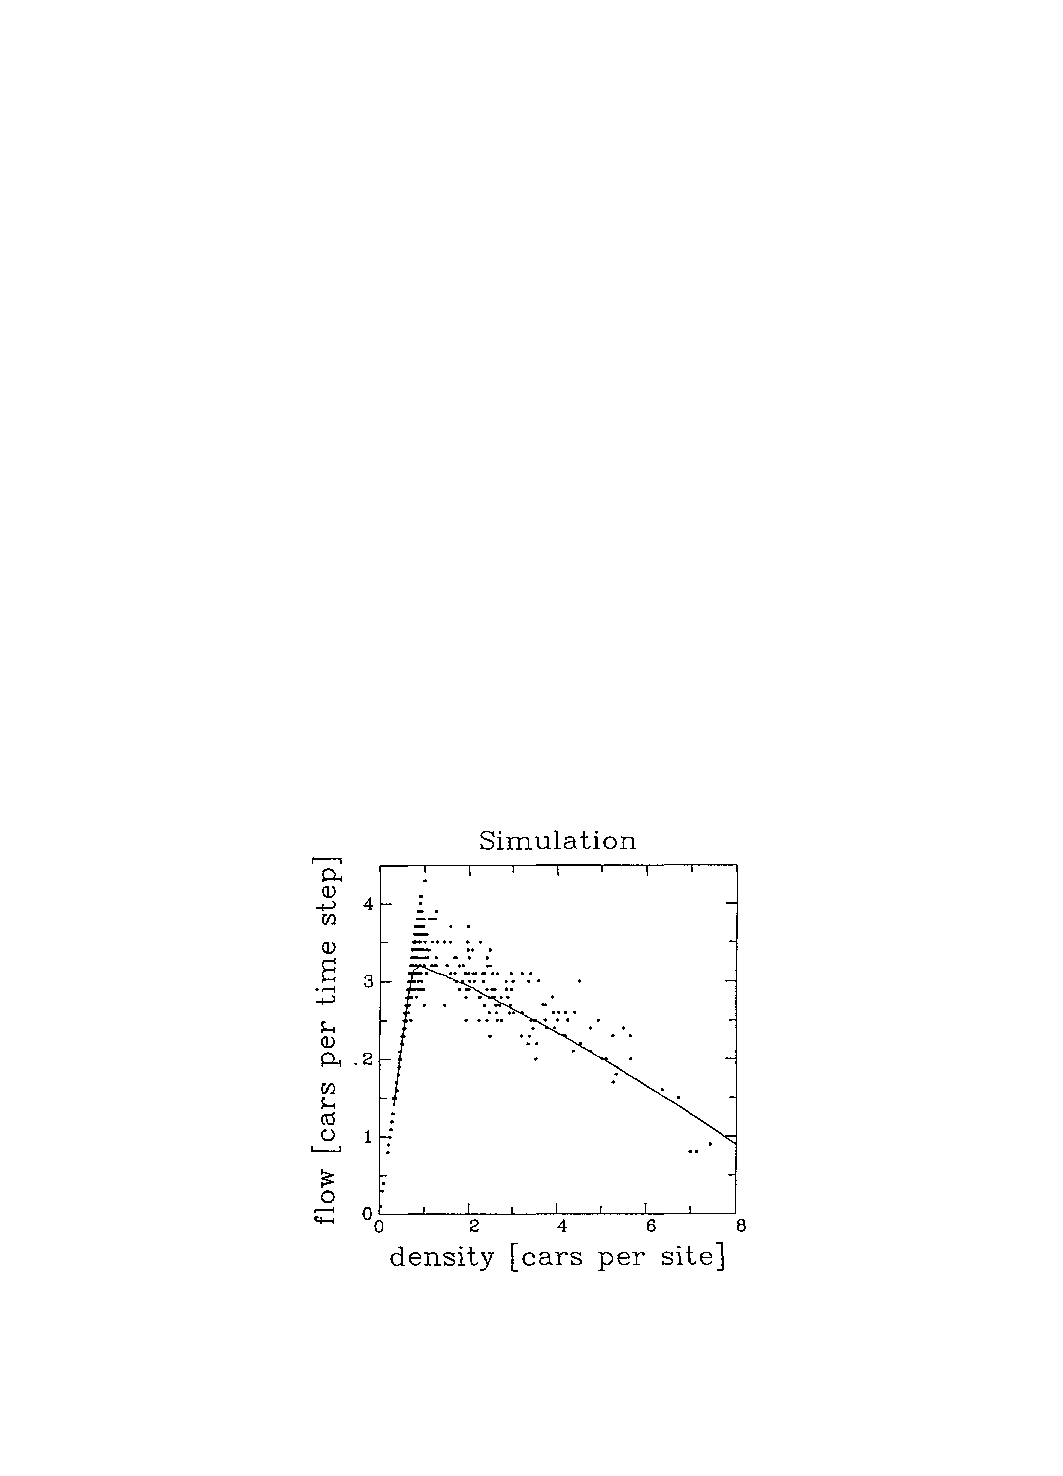
\includegraphics[scale = 0.7]{dfondcomp}
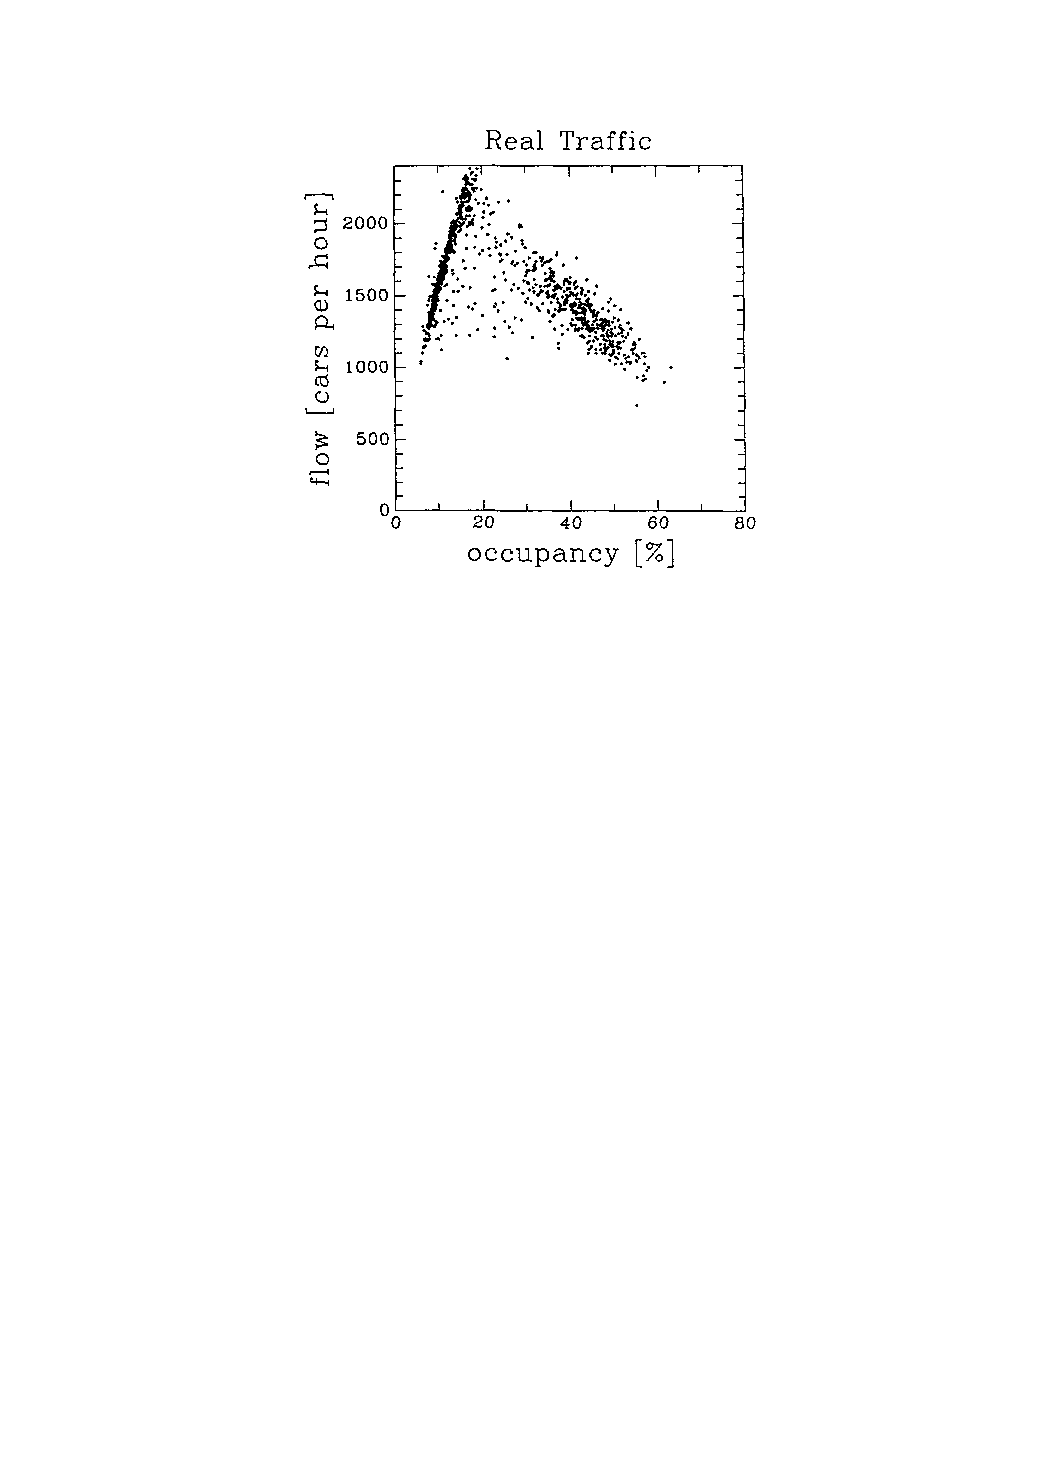
\includegraphics[scale = 0.7]{dfondcompre}
\end{frame}

\subsection{Intersections}
\begin{frame}
	\frametitle{intersection}
	Modèle Rui-Xiong, Ke-Zhao, Liu Mu-Ren
		\begin{equation}
			t_i = \frac{x_I - x_i}{\min(v_{max},d_i-1,v_i+1)}
		\end{equation}
\end{frame}
\end{document}